\begin{tikzpicture}
\node[inner sep=0pt] (obrazek) at (0,0)
    {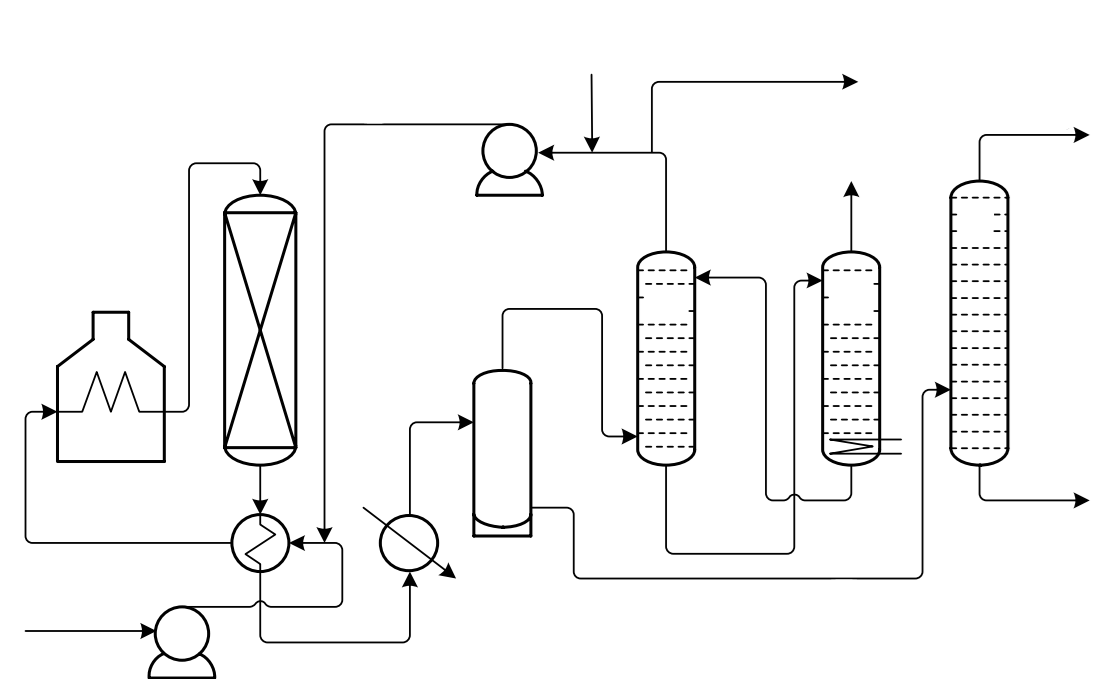
\includegraphics[width=0.8\textwidth]{figures/hydrogenr.png}};
\node[font=\small\bfseries] at (-3.75,-2.95) {1};
\node[font=\small\bfseries] at (-4.47,-0.885) {2};
\node[font=\small\bfseries] at (-2.95,1.1) {3};
\node[font=\small\bfseries] at (-0.475,-0.65) {4};
\node[font=\small\bfseries] at (1.2,0.4) {5};
\node[font=\small\bfseries] at (3.1,0.4) {6};
\node[font=\small\bfseries] at (4.4,1.25) {7};
\node[font=\small\bfseries] at (-0.4,2) {8};

\node[font=\small] at (-4.92,-3.15) {surovina};
\node[font=\scriptsize] at (-0.4,0.58) {vodíkový plyn};
\node[font=\scriptsize,align=center] at (-1.5,1.85) {cirkulační\\plyn};
\node[font=\scriptsize] at (0.45,2.96) {vodík};
\node[font=\scriptsize] at (2,2.96) {vodíkový plyn};
\node[font=\scriptsize] at (3.1,1.9) {sulfan};
\node[font=\scriptsize] at (1.9,-2.63) {kapalný produkt};
\node[font=\scriptsize,align=center] at (4.7,2.6) {\ce{C3} a \ce{C4}\\uhlovodíky};
\node[font=\scriptsize,align=center] at (4.8,-2.1) {odsířený\\produkt};
\end{tikzpicture}